\documentclass[10pt, xcolor={dvipsnames}]{beamer}
\usetheme{Boadilla}
\beamertemplatenavigationsymbolsempty
\setbeamerfont{title}{series=\bfseries}
\setbeamerfont{author}{series=\normalfont}
\setbeamerfont{frametitle}{series=\bfseries}
\setbeamerfont{footline}{series=\bfseries}
\setbeamertemplate{caption}[numbered]
\setbeamertemplate{page number in head/foot}{}
\usepackage{caption}

\definecolor{links}{HTML}{2A1B81}
\hypersetup{colorlinks,linkcolor=,urlcolor=links}
\setbeamercolor{bibliography item}{fg=black}
\setbeamercolor{bibliography entry author}{fg=black}
\setbeamercolor{bibliography entry title}{fg=black}
\setbeamercolor{bibliography entry location}{fg=black}
\setbeamercolor{bibliography entry note}{fg=black}

\usepackage[utf8x]{inputenc}
\usepackage[english]{babel}

\usepackage{graphicx}
%----------------------------------------------------------------------------------------
%	TITLE PAGE
%----------------------------------------------------------------------------------------

\setbeamerfont{title}{size=\large}
\setbeamerfont{author}{size=\normalsize}
\setbeamerfont{date}{size=\footnotesize}

\title[Toy Model]{Two Dimensional Toy Model and Layout Optimization}
\author[\textcolor{white}{Marko Lalovic}]{\textcolor{black}{Marko Lalovic} \vspace{-.7cm}}
\date[\textcolor{white}{July 12, 2022}]{\textcolor{black}{Summer 2022}}

\defbeamertemplate*{title page}{customized}[1][]
{
  \usebeamerfont{title}\inserttitle\par
  \usebeamerfont{subtitle}\usebeamercolor[fg]{subtitle}\insertsubtitle\par
  \bigskip
  \usebeamerfont{author}\insertauthor\par
  \usebeamerfont{institute}\insertinstitute\par
%  \usebeamerfont{date}\insertdate\par
  \usebeamercolor[fg]{titlegraphic}\inserttitlegraphic
  \bigskip
}
\newcommand{\norm}[1]{\left\lVert#1\right\rVert}

\begin{document}
\begin{frame}
\begin{center}
\maketitle
\begin{figure}
    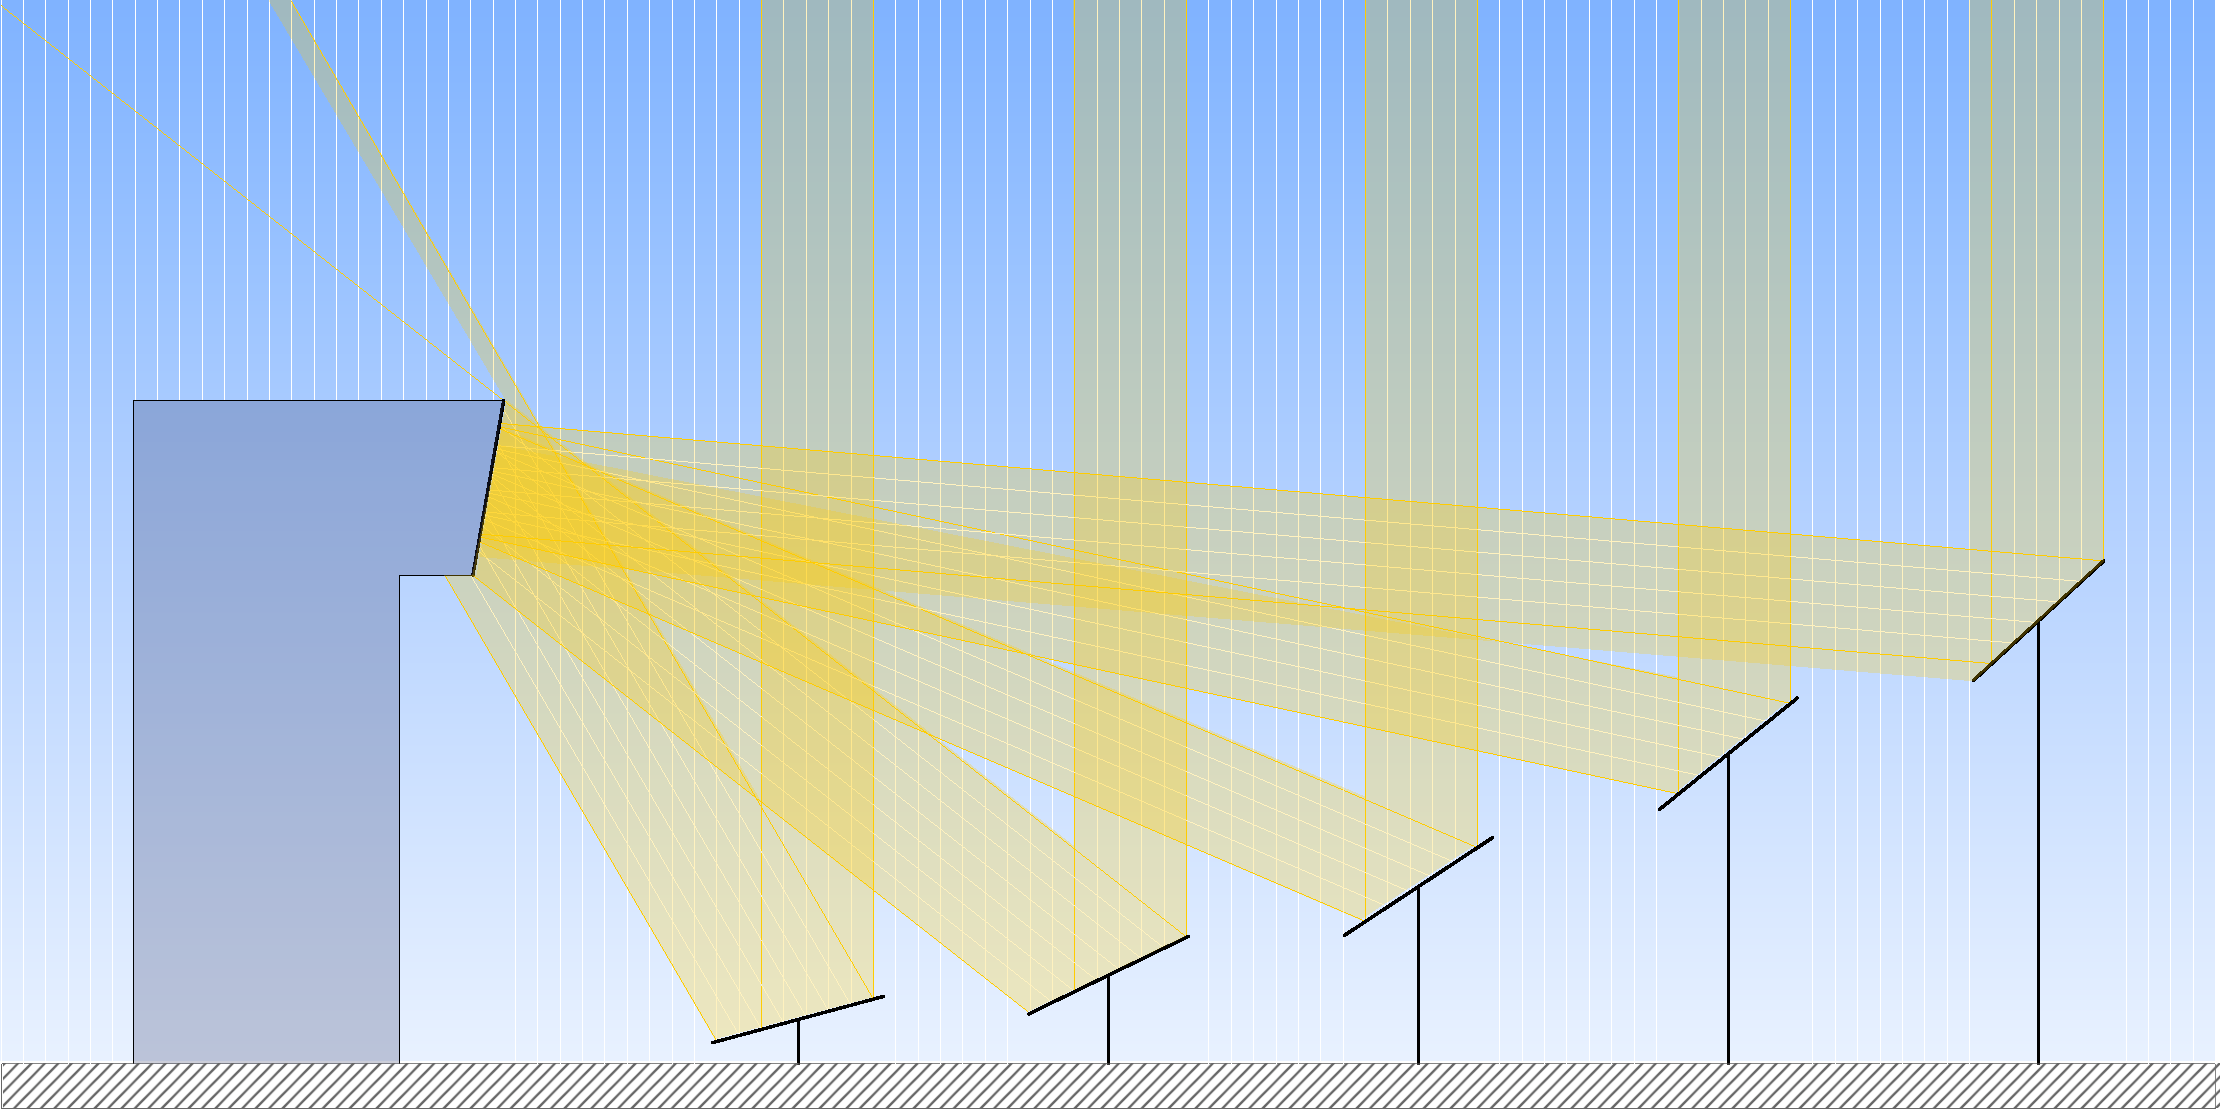
\includegraphics[width=\linewidth]{../figures/solar-toy-model-crop.pdf}
\end{figure}
\end{center}
\end{frame}

%----------------------------------------------------------------------------------------
%	PRESENTATION SLIDES
%----------------------------------------------------------------------------------------

\begin{frame}{Toy Model}

\begin{center}
\begin{figure}
\includegraphics[width=.95\textwidth]{../figures/states/toy-model-coords.png}
\caption{Model of a solar tower power plant in two dimensions}
\end{figure}
\end{center}
\end{frame}

\begin{frame}{Toy Model}
\begin{center}
\begin{figure}
\includegraphics[width=.95\textwidth]{../figures/states/toy-model/0.png}
\caption{Sun at 0°}
\end{figure}
\end{center}
\end{frame}

\begin{frame}{Toy Model}
\begin{center}
\begin{figure}
\includegraphics[width=.95\textwidth]{../figures/states/toy-model/1.png}
\caption{Sun at 30°}
\end{figure}
\end{center}
\end{frame}

\begin{frame}{Toy Model}
\begin{center}
\begin{figure}
\includegraphics[width=.95\textwidth]{../figures/states/toy-model/2.png}
\caption{Sun at 60°}
\end{figure}
\end{center}
\end{frame}

\begin{frame}{Toy Model}
\begin{center}
\begin{figure}
\includegraphics[width=.95\textwidth]{../figures/states/toy-model/3.png}
\caption{Sun at 90°}
\end{figure}
\end{center}
\end{frame}

\begin{frame}{Toy Model}
\begin{center}
\begin{figure}
\includegraphics[width=.95\textwidth]{../figures/states/toy-model/4.png}
\caption{Sun at 120°}
\end{figure}
\end{center}
\end{frame}

\begin{frame}{Toy Model}
\begin{center}
\begin{figure}
\includegraphics[width=.95\textwidth]{../figures/states/toy-model/5.png}
\caption{Sun at 150°}
\end{figure}
\end{center}
\end{frame}

\begin{frame}{Toy Model}
\begin{center}
\begin{figure}
\includegraphics[width=.95\textwidth]{../figures/states/toy-model/6.png}
\caption{Sun at 180°}
\end{figure}
\end{center}
\end{frame}

\begin{frame}{Layout Optimization}
\begin{center}
\begin{figure}
\includegraphics[width=.95\textwidth]{../figures/cos-effect-crop.pdf}
\caption{Cosine Effect}
\end{figure}
\end{center}
\end{frame}

\begin{frame}{Layout Optimization}
Using relations {\bf(c)} and {\bf(d)}
\begin{align*} %\frac{d}{d\rho}
\eta_{cos}(\rho) &= \int_{0}^{\pi} \cos \left( \frac{|\pi - \phi - \rho |}{2} \right) d\phi 
= 2 \left( \sin \left( \frac{\rho}{2} \right) 
+ \cos \left(\frac{\rho}{2}\right)  \right) \\[.5em]
\eta_{cos}'(\rho) &= \cos \left(\frac{\rho}{2}\right) - \sin \left( \frac{\rho}{2} \right) 
\implies \rho^{*} = \frac{\pi}{2}
\end{align*}

\begin{center}
\begin{figure}
\includegraphics[width=.95\textwidth]{../figures/spillage-problem-crop.pdf}
\caption{Spillage Effect}
\end{figure}
\end{center}
\end{frame}

\begin{frame}{Layout Optimization}
\begin{minipage}[t]{0.5\textwidth}
\begin{center}
\begin{figure}
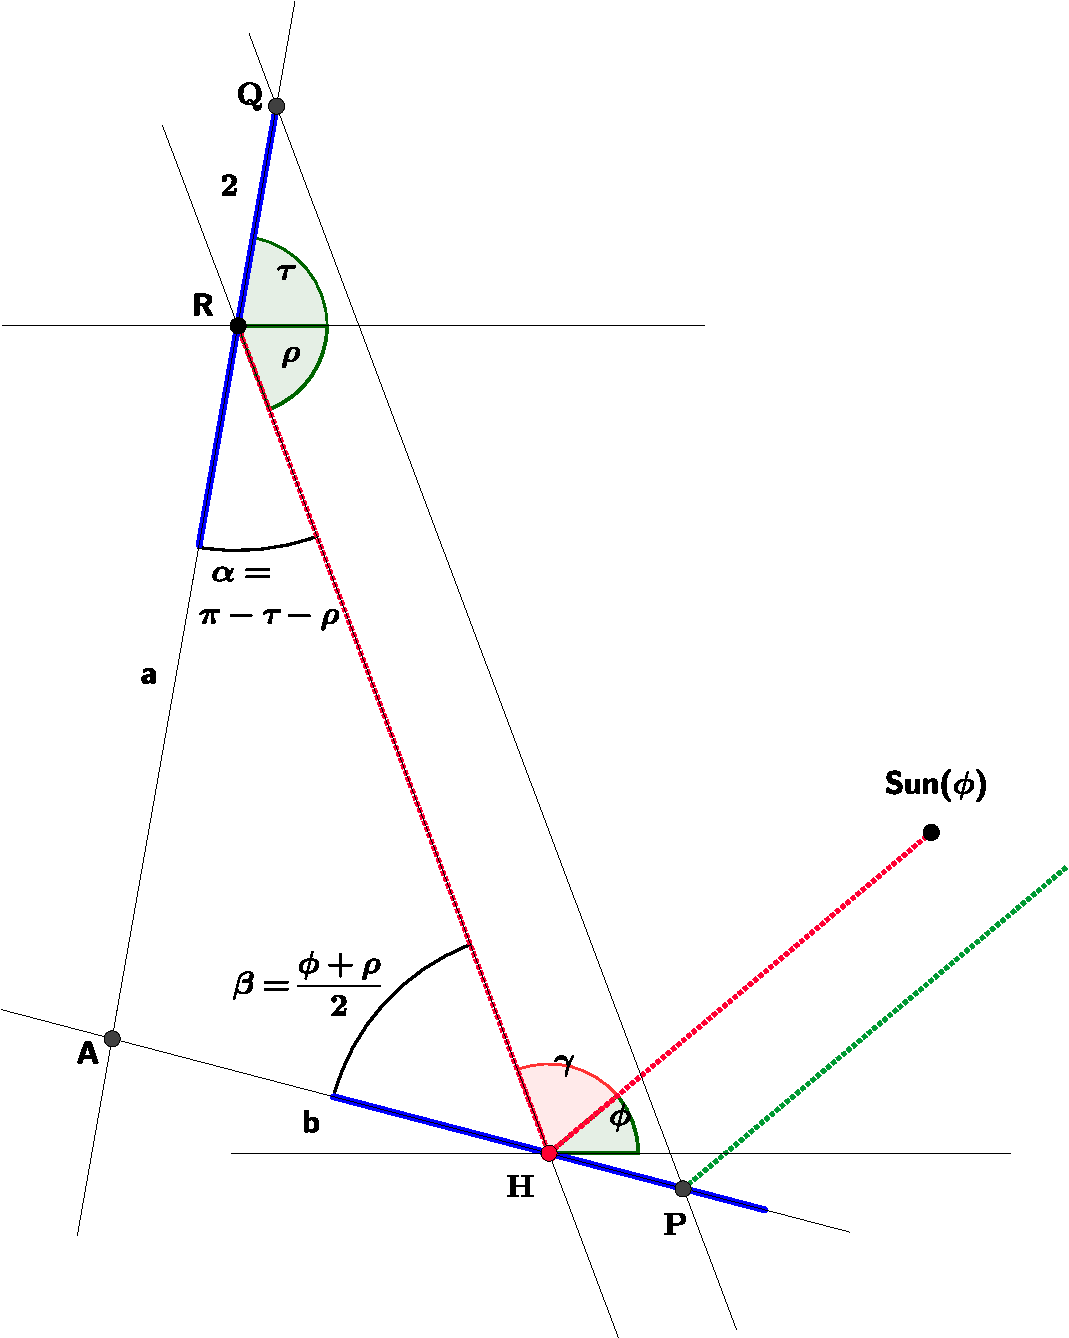
\includegraphics[width=.99\textwidth]{../figures/spillage-solving-crop.pdf}
\caption{Spillage Effect Solution}
\end{figure}
\end{center}
\end{minipage}%%%%%%%%%%%%%%%%
\begin{minipage}[t]{0.5\textwidth}
\vspace{2mm}
Using 
\begin{align*}
\frac{a + |RQ|}{a} &= \frac{b + |HP|}{b}
\quad \text{(Similarity)} \\[.5em]
\frac{a}{\sin(\alpha)} &= \frac{b}{\sin(\beta)}
\quad \text{(Sine Rule)}
\end{align*}
we get
\begin{align}
\eta_{spill} &= \min \left(1, \frac{|HP|}{2}\right) \\[.5em]
&= \min \left(1, 
\frac{\sin(\pi - \tau - \rho)}
{\sin \left( \frac{\phi + \rho}{2} \right)}
\right)
\end{align}
\end{minipage}
\end{frame}

\begin{frame}{Layout Optimization}
Let $d = \norm{H - R}$, then the {\it atmospheric attenuation}~\footnote{{\tiny \color{blue} P. Richter, Simulation and optimization of solar thermal power plants. PhD dissertation, RWTH Aachen University, 2017.}} is
\begin{equation}
\eta_{\text{aa}}(d_{i}) = \begin{cases}
0.99321 - 1.176 \cdot 10^{-4} d + 1.97 \cdot 10^{-8} d^{2}, \quad d \leq 1000 m\\
\exp(-1.106 \cdot 10^{-4} d), \quad d > 1000 m
\end{cases}
\end{equation}
\begin{center}
\begin{figure}
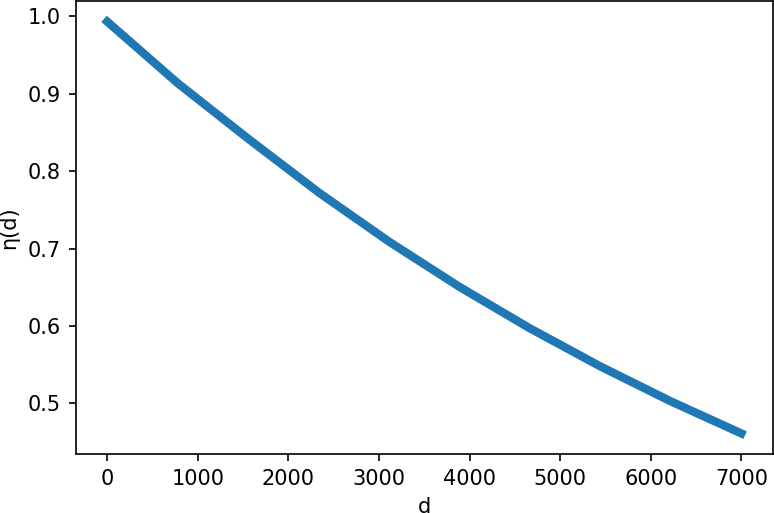
\includegraphics[width=.5\textwidth]{../figures/AA-crop.png}
\caption{Atmospheric Attenuation Effect}
\end{figure}
\end{center}
\end{frame}

\begin{frame}{Layout Optimization}
Let {\it Daily Energy Production} (DEP) be 
\begin{align}
\text{DEP}^{*} &= \int_{0}^{\pi} d\phi = \pi \\[.5em]
\text{DEP}(\rho, d) &= \eta_{aa}(d) \cdot 
\frac{1}{\pi}\int_{0}^{\pi} 
\eta_{cos}(\rho, \phi) \cdot \eta_{spill}(\rho, \phi)
d\phi
\end{align}
\begin{minipage}[t]{0.5\textwidth}
\begin{center}
\vspace{1.2cm}
\begin{figure}
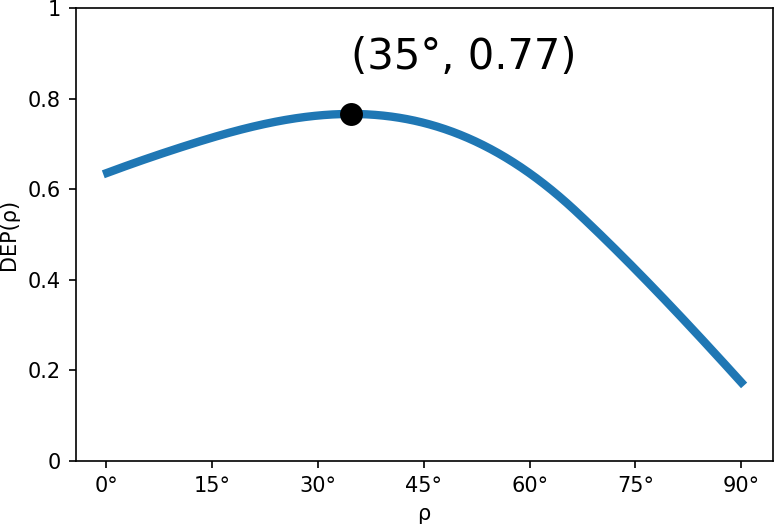
\includegraphics[width=.8\textwidth]{../figures/DEP-crop.png}
\caption{$\text{DEP}(\rho, d) = \text{DEP}(\rho)$.}
\end{figure}
\end{center}
\end{minipage}%%%%%%%%%%%%%%%%
\begin{minipage}[t]{0.5\textwidth}
\begin{center}
\begin{figure}
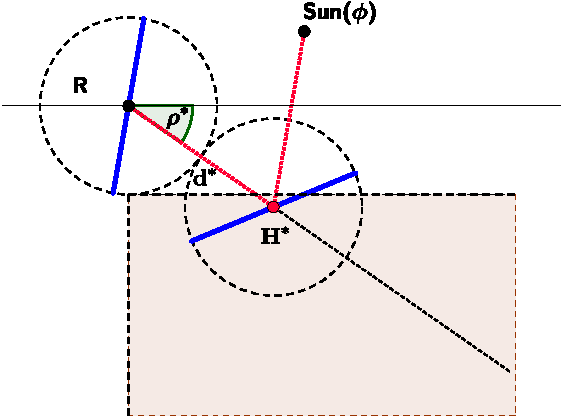
\includegraphics[width=\textwidth]{../figures/singleton-solution-crop.pdf}
\caption{Singleton Solution.}
\end{figure}
\end{center}
\end{minipage}
\end{frame}

\begin{frame}{Layout Optimization}
\begin{minipage}[t]{0.5\textwidth}
\begin{center}
\begin{figure}
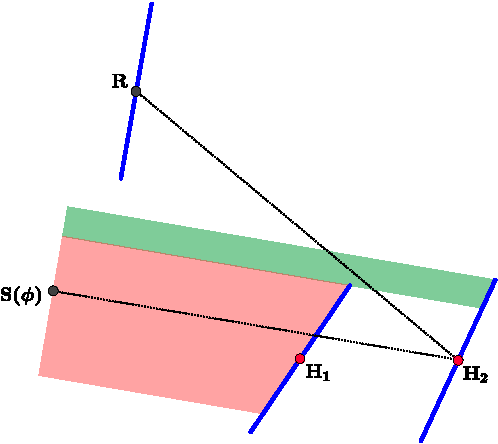
\includegraphics[width=.9\textwidth]{../figures/shading-crop.pdf}
\caption{Shading Effect.}
\end{figure}
\end{center}
\end{minipage}%%%%%%%%%%%%%%%%
\begin{minipage}[t]{0.5\textwidth}
\begin{center}
\begin{figure}
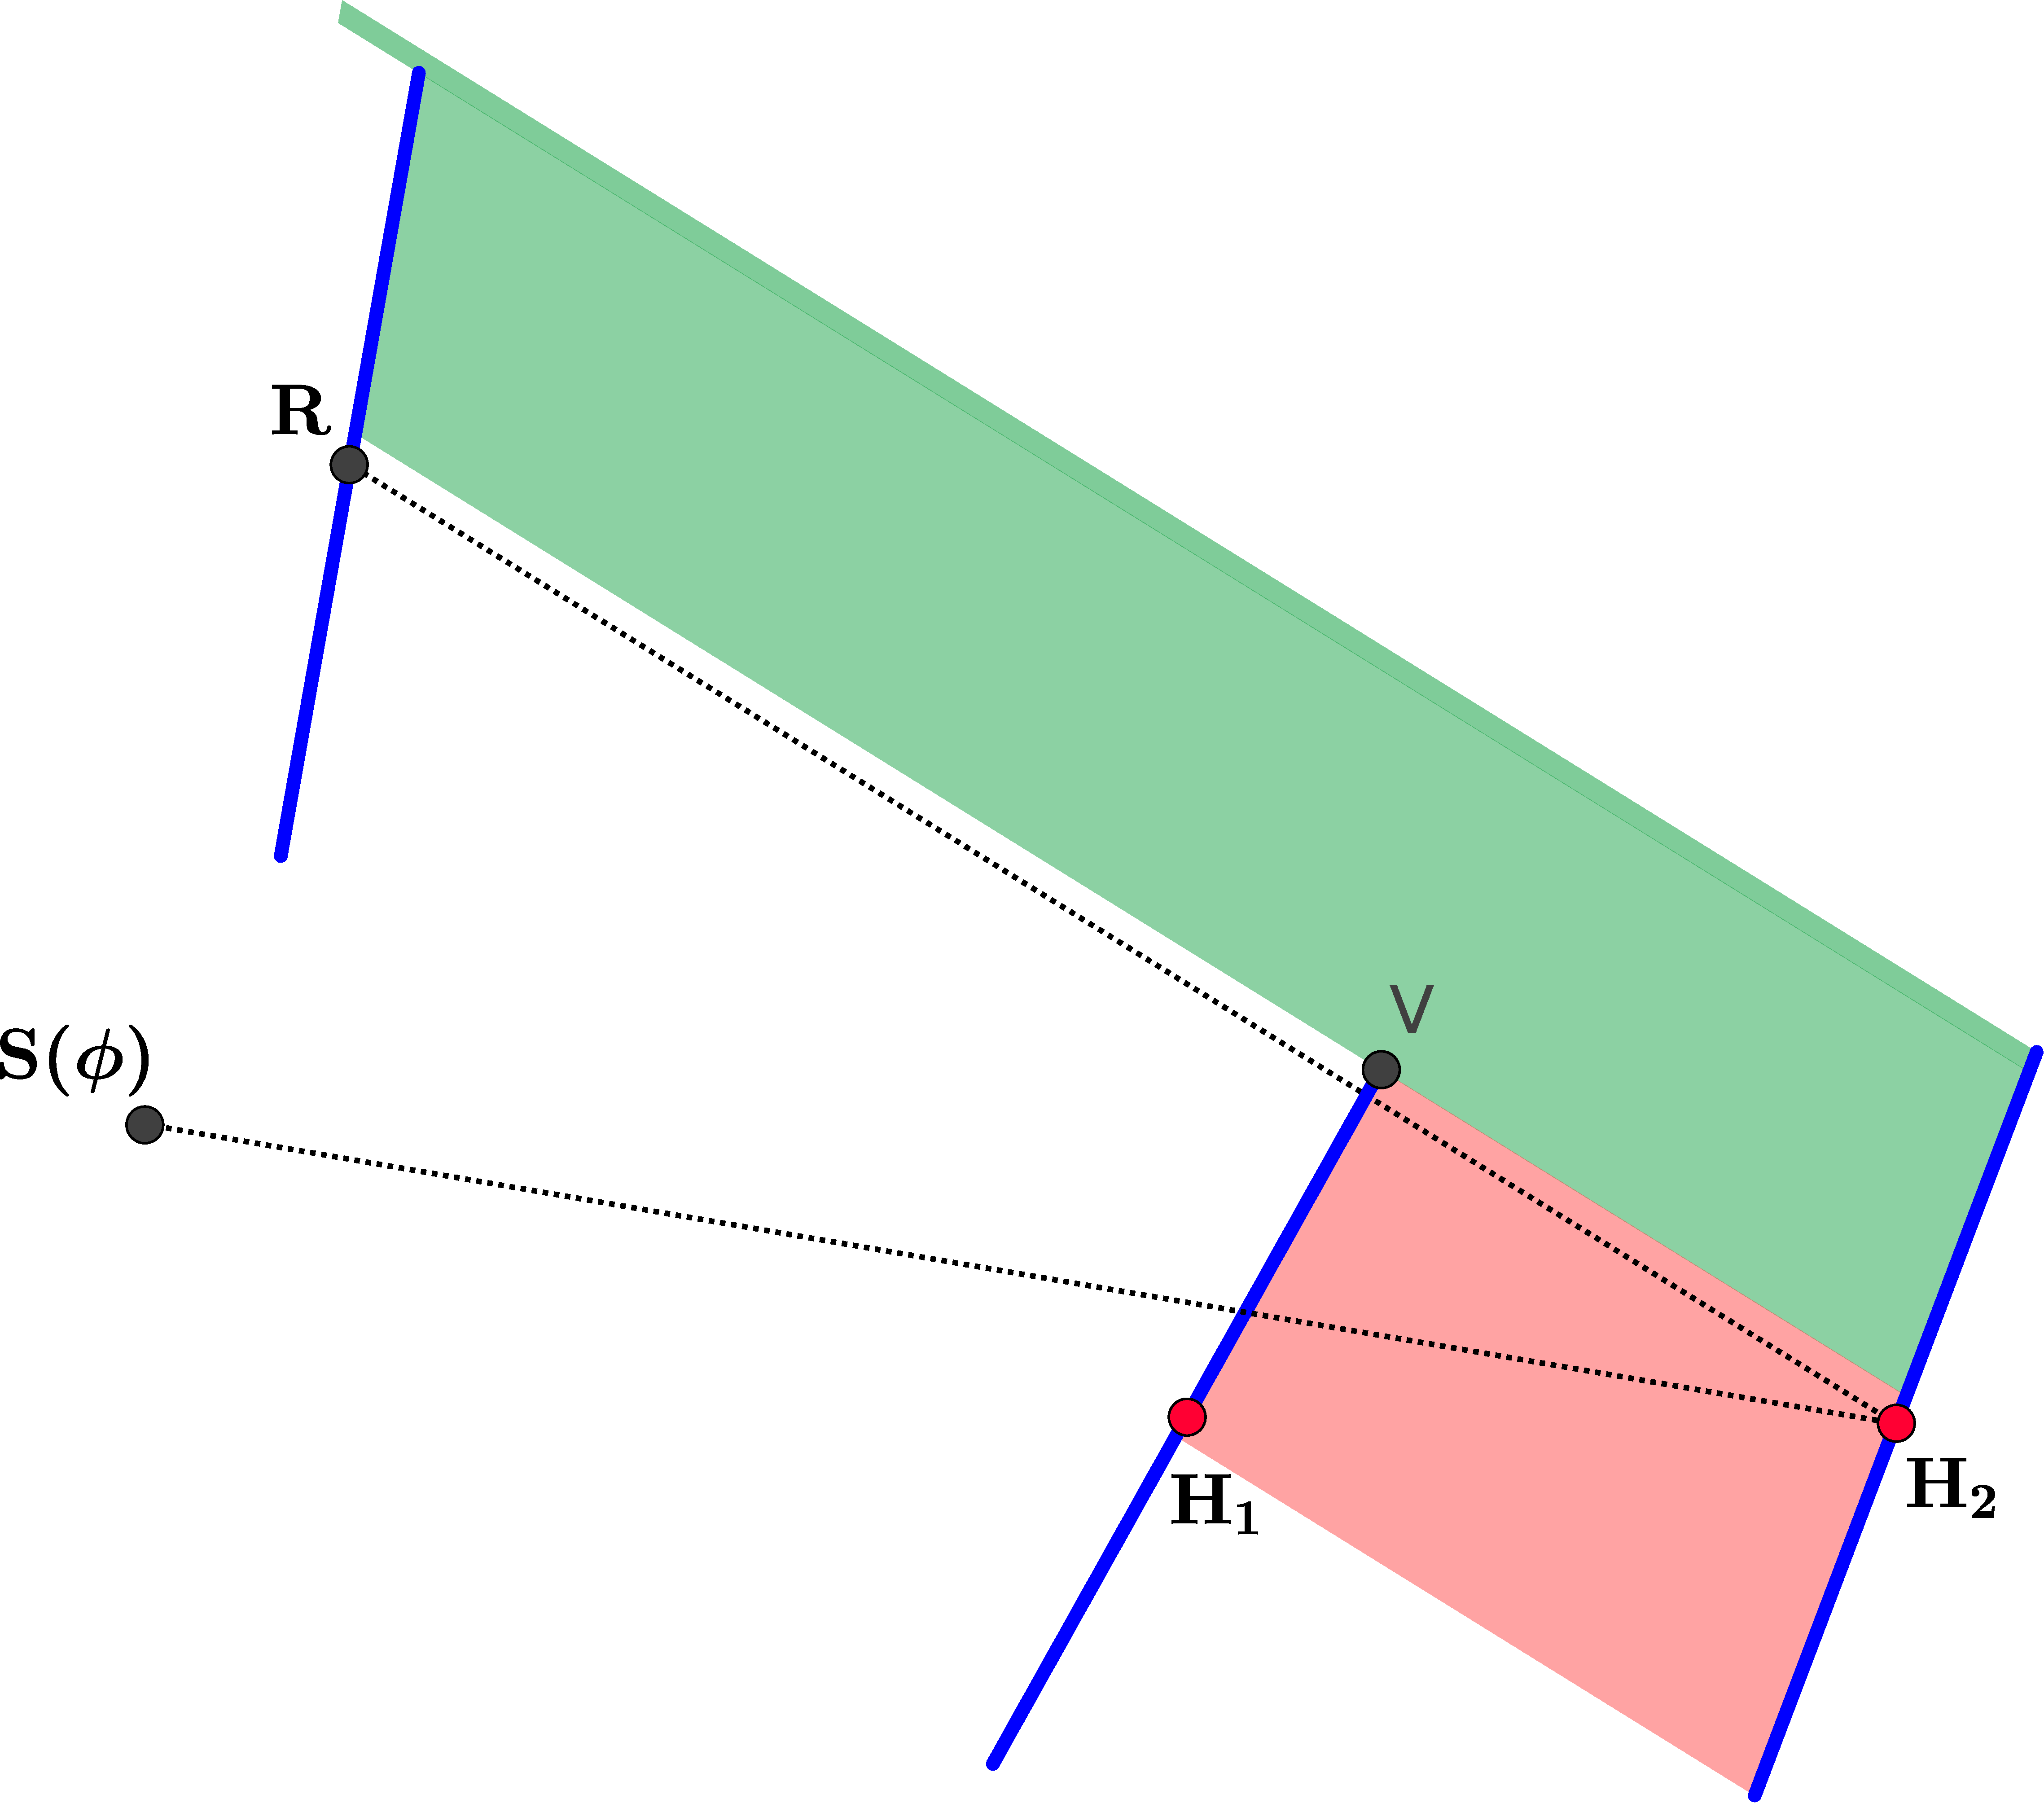
\includegraphics[width=.95\textwidth]{../figures/blocking-crop.pdf}
\caption{Blocking Effect.}
\end{figure}
\end{center}
\end{minipage}
\end{frame}

\begin{frame}{Layout Optimization}
For a given {\it layout} $H_{1}, H_{2}, \dots, H_{n}$
\begin{equation}
\widehat{\text{DAP}}(H_{1}, H_{2}, \dots, H_{n}) := 
\frac{1}{n\cdot m}
\sum_{i = 1}^{n} \eta_{aa} \cdot
\sum_{k = 1}^{m} \eta_{cos}(\phi_{k}) \cdot 
\eta_{ray}(\phi_{k})
\end{equation}
\vspace{-.4cm}
\begin{center}
\begin{figure}
\includegraphics[width=.4\textwidth]{../figures/layouts-old/tiny-layout-crop.png}
\end{figure}
\end{center}
\vspace{-0.4cm}
\begin{example}[Tiny Layout]
$$
H_1 = (6, 5), \quad 
H_2 = (12, 5), \quad
H_3 = (18, 5), \quad
H_4 = (23, 5), \quad
H_5 = (29, 5)
$$
Using $m = 17$ and $5$ rays per heliostat we get $\widehat{\text{DAP}} \approx 0.53$~\footnote{Found one error in the code, but the results do not change significantly so I'm showing the same results as in the Report.}
\end{example}
\end{frame}

\begin{frame}{Layout Optimization}
\begin{minipage}[t]{0.5\textwidth}
\begin{center}
\begin{figure}
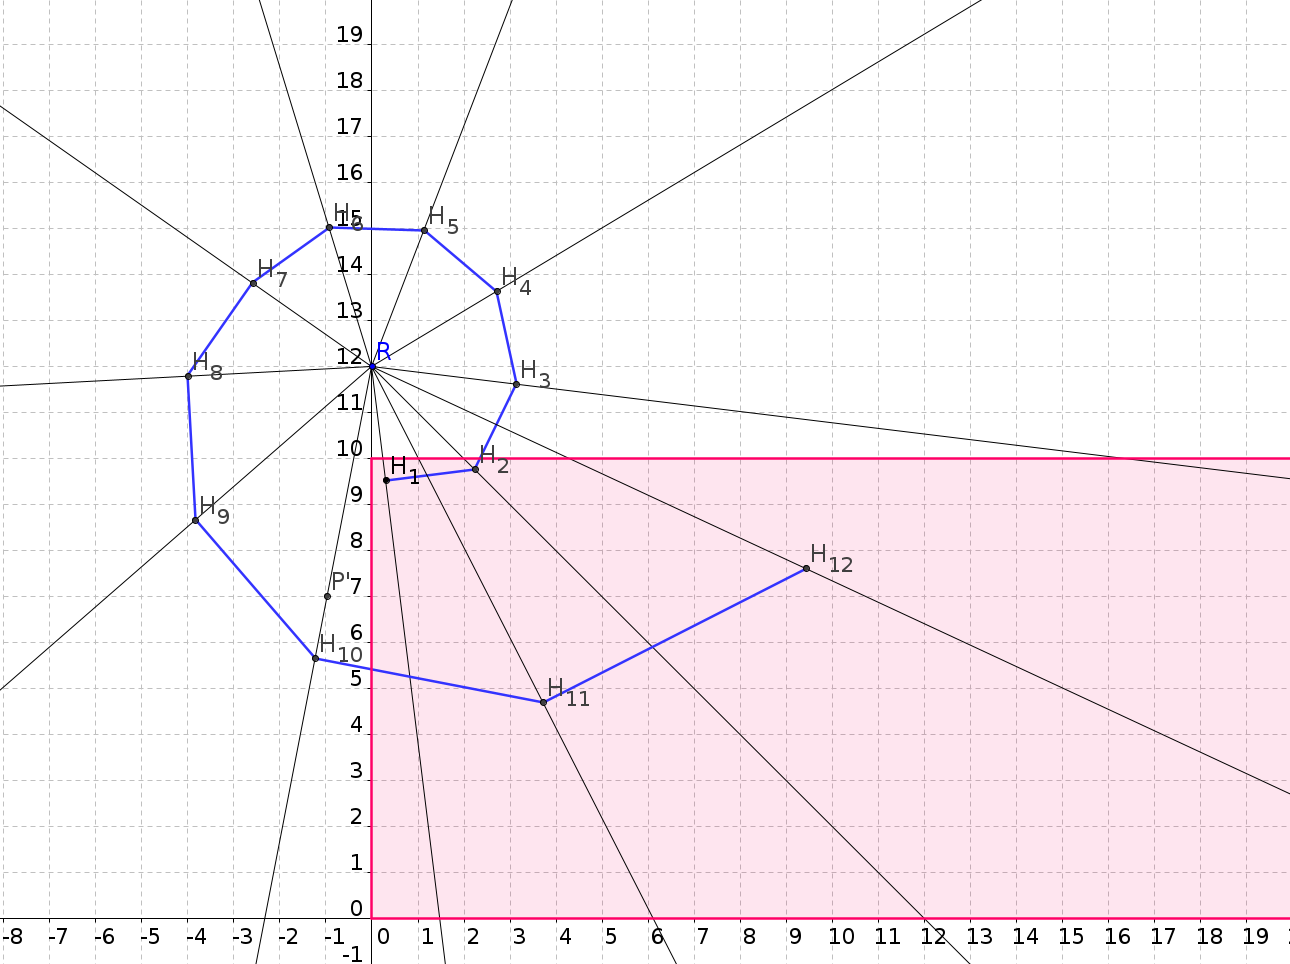
\includegraphics[width=\textwidth]{../figures/spiral/spiral-construction.png}
\caption{Spiral idea.}
\end{figure}
\end{center}
\end{minipage}%%%%%%%%%%%%%%%%
\begin{minipage}[t]{0.5\textwidth}
\begin{center}
\vspace{-.5cm}
\begin{figure}
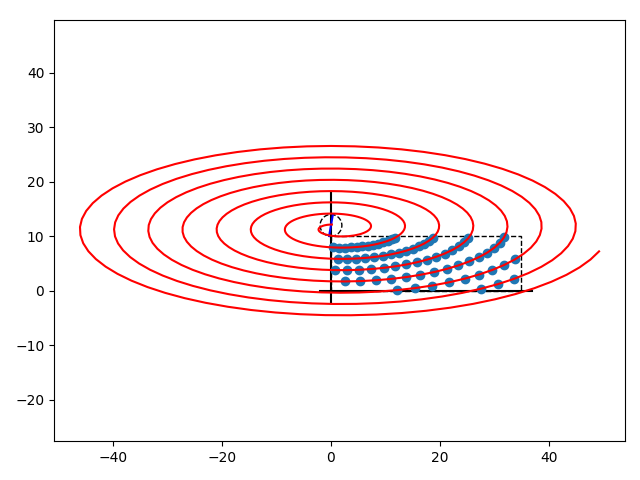
\includegraphics[width=\textwidth]{../figures/spiral/spiral_plot.png}
\caption{Possible heliostat positions.}
\end{figure}
\end{center}
\end{minipage}
\begin{center}
\begin{figure}
\includegraphics[width=.35\textwidth]{../figures/layouts-old/spiral-layout-crop.png}
\caption{Spiral Layout that ``grew up on the spiral".}
\end{figure}
\end{center}
\end{frame}

\begin{frame}{Layout Optimization}
Placing the heliostats equidistantly some distance apart on the parabola
\begin{equation}
y = \frac{1}{48} x^{2}
\end{equation}
with the focal point $R = (0, 12)$
\begin{minipage}[t]{0.5\textwidth}
\begin{center}
\begin{figure}
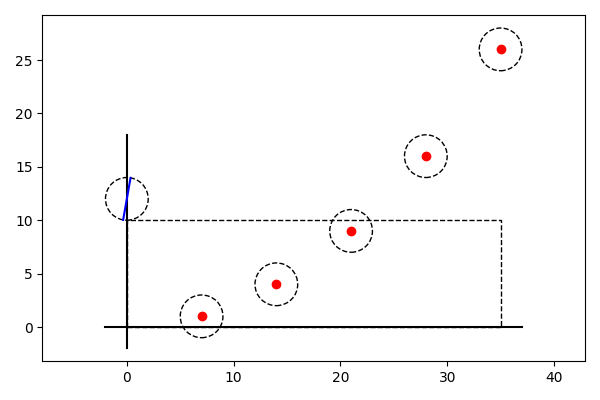
\includegraphics[width=\textwidth]{../figures/layouts-old/parabolic-mirror-layout.png}
\caption{Parabolic Mirror Layout.}
\end{figure}
\end{center}
\end{minipage}%%%%%%%%%%%%%%%%
\begin{minipage}[t]{0.5\textwidth}
\begin{center}
\begin{figure}
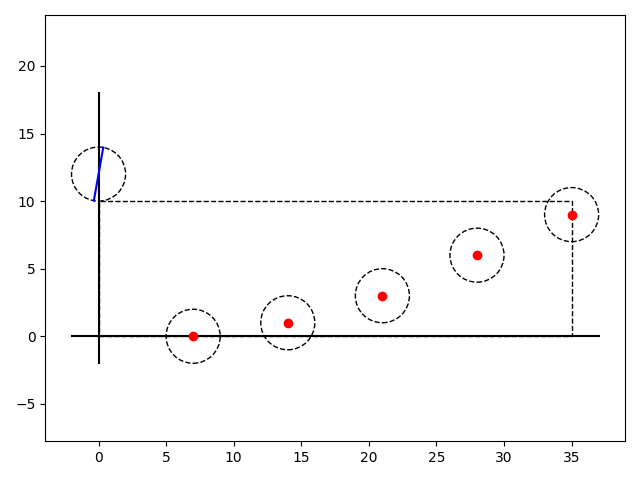
\includegraphics[width=.9\textwidth]{../figures/layouts-old/parabolic-layout-2.png}
\caption{Valid Parabolic Layout.}
\end{figure}
\end{center}
\end{minipage}
\end{frame}

\begin{frame}{Layout Optimization}
Plots of $\widehat{\text{DAP}}(x_3, y_3)$
\begin{minipage}[t]{0.5\textwidth}
\begin{center}
\begin{figure}
\includegraphics[width=.9\textwidth]{../figures/landscape/surface_plot_rotated-old.png}
\caption{Landscape.}
\end{figure}
\end{center}
\end{minipage}%%%%%%%%%%%%%%%%
\begin{minipage}[t]{0.5\textwidth}
\begin{center}
\vspace{-.5cm}
\begin{figure}
\includegraphics[width=.9\textwidth]{../figures/landscape/surface_plot-old.png}
\caption{Landscape rotated.}
\end{figure}
\end{center}
\end{minipage}
\end{frame}

\begin{frame}{Layout Optimization}
Running gradient ascent
\begin{equation}
x_{k} = x_{k - 1} + \sigma \cdot g
\end{equation}
where $g$ is first finite difference estimate and $\sigma = 1$
\begin{minipage}[t]{0.5\textwidth}
\begin{center}
\begin{figure}
\includegraphics[width=\textwidth]{../figures/landscape/gradient_ascent_close-old.png}
\caption{Starting close to the optimum.}
\end{figure}
\end{center}
\end{minipage}%%%%%%%%%%%%%%%%
\begin{minipage}[t]{0.5\textwidth}
\vspace{0.1cm}
\begin{center}
\begin{figure}
\includegraphics[width=\textwidth]{../figures/landscape/gradient_ascent_far-old.png}
\caption{Starting far from the optimum.}
\end{figure}
\end{center}
\end{minipage}
\end{frame}

\begin{frame}{Layout Optimization}
Running gradient ascent
\begin{equation}
x_{k} = x_{k - 1} + \sigma \cdot g
\end{equation}
where $g$ is first finite difference estimate and $\sigma = 1$
\begin{minipage}[t]{0.5\textwidth}
\begin{center}
\begin{figure}
\includegraphics[width=\textwidth]{../figures/landscape/gradient_ascent_close-old.png}
\caption{Starting close to the optimum.}
\end{figure}
\end{center}
\end{minipage}%%%%%%%%%%%%%%%%
\begin{minipage}[t]{0.5\textwidth}
\vspace{0.1cm}
\begin{center}
\begin{figure}
\includegraphics[width=\textwidth]{../figures/landscape/gradient_ascent_far-old.png}
\caption{Starting far from the optimum.}
\end{figure}
\end{center}
\end{minipage}
\end{frame}

\begin{frame}{Layout Optimization}
Running Sequential Quadratic Programming (SQP) method, from a class of Lagrange-Newton methods
\begin{minipage}[t]{0.5\textwidth}
\begin{center}
\begin{figure}
\includegraphics[width=\textwidth]{../figures/landscape/sqp-test-1.png}
\caption{Initial value.}
\end{figure}
\end{center}
\end{minipage}%%%%%%%%%%%%%%%%
\begin{minipage}[t]{0.5\textwidth}
\vspace{0.15cm}
\begin{center}
\begin{figure}
\includegraphics[width=\textwidth]{../figures/landscape/sqp-test-2.png}
\caption{Converged.}
\end{figure}
\end{center}
\end{minipage}
\end{frame}

\begin{frame}{Layout Optimization}
Running a set of different methods
\begin{center}
\begin{figure}
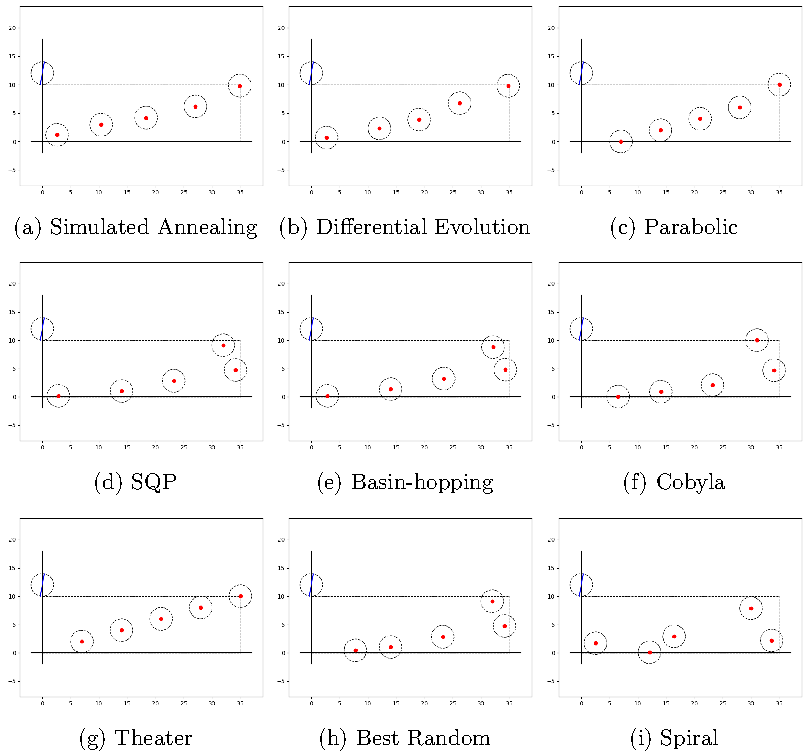
\includegraphics[width=.64\textwidth]{../figures/layouts/layouts.pdf}
\caption{Top 9 Layouts.}
\end{figure}
\end{center}
\end{frame}

\begin{frame}{Layout Optimization}
\begin{itemize}
\item Most layouts were only exploiting the inaccuracies in the Toy model
\item Increasing the number of angles from 17 to 180 and rays from 5 to 50:
\end{itemize}

\begin{table}
\parbox{.45\linewidth}{
\centering
\begin{tabular}{lllll}
              &  $\widehat{\text{DAP}}$    &  &  &  \\
annealing-layout    & 0.77 &  &  &  \\[.5em]
de-layout           & 0.77 &  &  &  \\[.5em]
parabolic-layout    & 0.74 &  &  &  \\[.5em]
basinhopping-layout & 0.72 &  &  &  \\[.5em]
sqp-layout          & 0.72 &  &  &  \\[.5em]
cobyla-layout       & 0.72 &  &  &  \\[.5em]
theater-layout      & 0.71 &  &  &  \\[.5em]
random-layout       & 0.70 &  &  &  \\[.5em]
spiral-layout       & 0.66 &  &  & 
\end{tabular}
\caption{Layout optimization accuracy.}
}
\hfill
\parbox{.45\linewidth}{
\centering
\begin{tabular}{lllll}
              &  $\widehat{\text{DAP}}$    &  &  &  \\
parabolic-layout    & 0.80 &  &  &  \\[.5em]
annealing-layout    & 0.77 &  &  &  \\[.5em]
de-layout           & 0.77 &  &  &  \\[.5em]
theater-layout      & 0.77 &  &  &  \\[.5em]
cobyla-layout       & 0.76 &  &  &  \\[.5em]
random-layout       & 0.75 &  &  &  \\[.5em]
basinhopping-layout & 0.73 &  &  &  \\[.5em]
sqp-layout          & 0.73 &  &  &  \\[.5em]
spiral-layout       & 0.66 &  &  &  
\end{tabular}
\caption{Increased model accuracy.}
}
\end{table}
\end{frame}

\begin{frame}{TODOs and Open Questions}
\begin{itemize}
\item Improve the model and repeat the optimization and evaluation
\item Try showing that putting heliostats on parabola is the best layout
\item Contribute github.com/markolalovic/math-mods-camp
\end{itemize}

\begin{center}
\begin{figure}[H]
\includegraphics[width=.6\textwidth]{../figures/proof2.png}
\caption{Minimizing the effects of shading and blocking.}
\end{figure}
\end{center}

\end{frame}

\end{document}